\section{Canonical T-Action and Generalization of Delzant's Theorem}

In this last section, we were studying the fibre  $\pi: P \to \mathcal{O}$, and we noted that the transition functions between fibres were contained in a fundamental torus $G_{\mu}$. Now, we want to use this fact to develop an $S^{1}$-action on fibres. This twisted $S^{1}$-action will allow us to develop a Delzant-type correspondence, where when we compare two manifolds, if the $S^{1}$-spaces arising via bundle fibres are symplectomorphic via the twisted $S^{1}$-action, then the corresponding Hamiltonian $\mathrm{SO}(3)$-spaces are equivariant symplectomorphic. In this section, we will:
\begin{enumerate}
    \item Develop a framework for the twisted $S^{1}$-action.
    \item Prove a version of Delzant's Theorem.
\end{enumerate}
\subsection{Construction of the Twisted $S^1$-Action}
Recall how the transition functions arising from the $\pi$ bundle acted. On each fibre $\pi^{-1}(\mu)$ there is the group action $G_{\mu}$. Now, we consider the group isomorphism:
\begin{align}
k_{\mu}: S^{1} \to G_{\mu} \text{ where } \mu = g \cdot \mu_{0} && \text{ given by } k_{\mu}(t) \mapsto gtg^{-1} 
\end{align}

\noindent This allows us to define an $T$-action $\bullet$ on $P$ given by: 

\begin{defn}[$T$-action on $P$]
Let $(P, \omega, \rm{SO}(3))$ be a symplectic manifold with Hamilitonian Lie action. Then, a twisted $T$ action $T \circlearrowleft P$ is given by:

\begin{equation}
t \bullet x = k_{\pi(x)}(t) \cdot x
\end{equation}

\noindent Where $k_{\mu}(t) \mapsto gtg^{-1}$, and $T$ is the maximum tori of $\rm{SO}(3)$.
\end{defn}

\begin{remark}
We say that $T$ acts on $x$ via a twisted action $k_{\pi(x)}$, which is manifestly abelian. By definition, the generators of this action are:
\end{remark}

\begin{defn}[Infinitesimal generators of $T$ action]
The infinitesimal generators are:

\begin{equation}
\xi_{P} = \lim_{\tau \to 0} \frac{d}{d \tau} \exp(\tau \xi) \bullet x
\end{equation}
\end{defn}

\begin{lemma}[Generators of $T$-action]
The infinitesimal generators of $T = S^{1}$ and $G = \mathrm{SO}(3)$ are related for any $\xi \in \mathfrak{t} \subset \mathfrak{g}$ by:
\begin{equation}
\xi_{P}^{T}(x) = (\mathrm{Ad}_{g} \xi)_{P} (x)
\end{equation}
\end{lemma}

\begin{proof}
This follows by derivation of the above $\bullet$ definition. Take the derivative of $\exp(t \xi) \cdot x$:
\begin{align}
\xi_{P}^{T} &= \lim_{\tau \to 0} \frac{d}{d \tau} g \exp(\tau \xi) g^{-1}\\
\xi_{P}^{T} &= \mathrm{Ad}_{g} \xi
\end{align}
Where $\mu = g \cdot \mu_{0}$, or $\pi(x) = g \cdot \mu_{0} \Longleftrightarrow g^{-1} \cdot x \in \pi^{-1}(\mu_{0})$.
\end{proof}

\begin{theorem}[\textcite{Blaom1996}]\label{thm:t-action-hamiltonian}
The $T$ action defined above is Hamiltonian. Furthermore, a $T$-equivariant moment map for this action is $j = i \circ \pi_{\mathcal{W}} \circ J$ 
\end{theorem}

\begin{proof}
We want to show:
\begin{equation}
\langle dj_{x'} v, \xi \rangle = \langle dJ_{x'} v, \mathrm{Ad}_{g} \xi \rangle
\end{equation}
when $v \in \operatorname{Hor}_{x}$ and when $v \in T_{x} \pi^{-1}(\mu)$. As these are $\omega$-orthogonal, that will imply that:
\begin{equation}
\langle dj_{x'} v, \xi \rangle = \langle dJ_{x'} v, \mathrm{Ad}_{g} \xi \rangle
\end{equation}
everywhere. Moreover, this will prove that $T$ is Hamiltonian with the infinitesimal generators:
\begin{equation}
X_{j_{\xi}} = \xi_{P}^{T}(x)
\end{equation}
Let's prove the first part - note that $j$ is $G$-invariant, since orbits factor out under $\pi_{\mathcal{W}}$. Since the $T \trianglelefteq G$ action is trivial, we also have $j$ is $T$-equivariant. For fixed $\mu_{0}$, choose $\mu = \pi(x) = g \cdot \mu_{0}$, and note that for the Weyl chamber $\mathcal{W}$, $g^{-1} J(x') \in \mathcal{W}$. Now, for any $\xi \in \mathfrak{t}$, we note that $g^{-1} J(x')$ survives the projection $\pi_{\mathcal{W}}$. 
\begin{equation}
\langle j(x'), \xi \rangle = \langle \pi_{\mathcal{W}} J(x'), \xi \rangle = \langle g^{-1} \cdot J(x'), \xi \rangle
\end{equation}
Taking derivatives of both sides, we have:
\begin{equation}
\langle dj_{x'} v, \xi \rangle = \langle dJ_{x'} v, \mathrm{Ad}_{g} \xi \rangle
\end{equation}
In particular, this occurs when $x' \in T_{x} \pi^{-1}(\mu)$.
\end{proof}
\begin{lemma}\label{lem:derivatives-vanish}
Both the derivative of $j$ and the derivative of $J$ vanish on horizontal fibres:
\begin{equation}
\{\langle dJ_{x'} v, \mathrm{Ad}_{g} \xi \rangle: v \in \operatorname{Hor}_{x} \} = 0
\end{equation}
\end{lemma}
\begin{proof}
Firstly, since $j$ is $G$-invariant, yet elements of $\operatorname{Hor}_{x}$ live in the domain $T_{x}(G \cdot x)$, we conclude that $\{\langle dj_{x'} v, \xi \rangle: v \in \operatorname{Hor}_{x} \} = 0$. Now, to show that the derivative of $J$ vanishes, note that $dJ_{x'} v$ must be tangent to the coadjoint orbit through $x$, so that:
$dJ_{x'} v = \mathrm{ad}_{\nu} J(x')$. Then:
\begin{align}
\langle dJ_{x'} v, \mathrm{Ad}_{g} \xi \rangle &= \langle \mathrm{ad}_{\nu} J(x'), \mathrm{Ad}_{g} \xi \rangle\\
&= \langle J(x'), [\nu, \mathrm{Ad}_{g} \xi] \rangle\\
&= \langle \mathrm{Ad}_{g}^{*} J(x'), [\mathrm{Ad}_{g^{-1}} \nu, \xi] \rangle\\
&= -\langle \mathrm{ad}^{*}_{\xi} \left[ g^{-1} \cdot J(x') \right], \mathrm{Ad}_{g^{-1}} \nu \rangle
\end{align}
Since $g^{-1} J(x') \in \mathcal{W}$, $\mathrm{ad}^{*}_{\xi} \left[ g^{-1} \cdot J(x') \right] = 0$, the conclusion follows.
\end{proof}
\begin{lemma}[Classical] \label{lem:local-sections}
If $G$ is a Lie group and $H$ a closed subgroup of $G$, then $G \to G/H$ is a principal $G$ bundle.
\end{lemma}
We will use this lemma to build charts for a symplectomorphism on the $G = \mathrm{SO}(3)$ level between manifolds. 

\noindent \textbf{References}: \textcite{Blaom1996}

\subsection{Equivalence of Hamiltonian G-Spaces}
\begin{theorem}\label{thm:hamiltonian-g-spaces-equivalence}
Let $G$ be a compact, connected Lie group. Then two Hamiltonian $G = \rm{SO}(3)$-spaces with regular momenta are equivalent if and only if their associated $T$-spaces are equivalent.
\end{theorem}
\begin{proof}
The forward direction is clear. Let $(P_{1}, \omega_{1}, G, J^{1})$ and $(P_{2}, \omega_{2}, G, J^{2})$ be Hamiltonian $G$-spaces. We have symplectic fibrations $\pi_{1}: P_{1} \to \mathcal{O}$ and $\pi_{2}: P_{2} \to \mathcal{O}$. Let $F_{1}$ and $F_{2}$ be fibres of $\pi_{1}$ and $\pi_{2}$ over $\mu_{0}$ respectively, where $\mu_{0}$ is just a choice $\mu_{0} \in \mathfrak{g}_{reg}^{*}$. Let's assume we have a $T$-equivariant symplectomorphism:
\begin{align}
\varphi&: F_{1} \to F_{2}\\
J^{F_{2}} \circ \varphi &= J^{F_{1}}
\end{align}
Let $x \in P_{1}$ such that $\pi_{1}(x) = g \cdot \mu_{0}$. Define:
\begin{equation}
\phi(x) = g \cdot \varphi(g^{-1} \cdot x)
\end{equation}

\begin{figure}
    \centering
    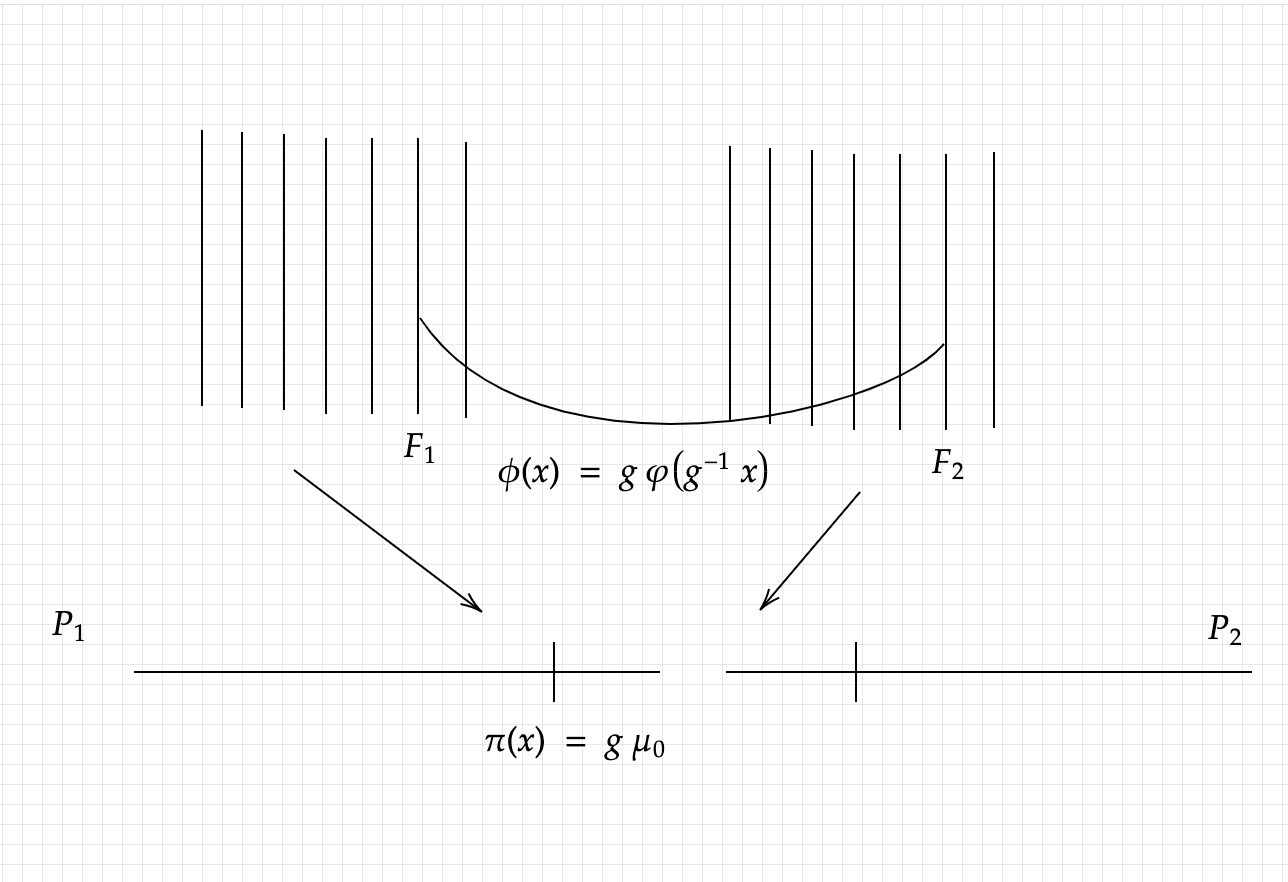
\includegraphics[width=0.5\linewidth]{Chapters/Figures/w.png}
    \caption{To move between fibres, we define $\phi(x) = g \cdot \varphi(g^{-1} \cdot x) $} 
    \label{fig:enter-label}
\end{figure}


\noindent It suffices to show that $\phi$ is well-defined, $\phi$ is $G$-equivariant and $J^{2} \circ \phi = J^{1}$, and there exists an inverse for $\phi$.
\end{proof}
\begin{lemma}\label{lem:phi-well-defined}
$\phi(x)$ is well defined, for a choice of $g \in G$.
\end{lemma}
\begin{proof}
We consider $g$ such that $g \cdot \mu_{0} = \mu_{0}$. Note that $g \cdot \mu_{0}$ is unique up to a factor of $g \cdot t$, where $t \in G_{\mu_{0}}$. Now we note that $\phi(x)$ does not depend on $g$:
\begin{align}
\phi(x) &= gt \cdot \varphi(t^{-1} \circ g^{-1} \cdot x)\\
\phi(x) &= g \cdot \varphi(g^{-1} \cdot x)
\end{align}
\end{proof}
\begin{lemma}\label{lem:phi-equivariant}
$\phi$ is $G$-equivariant. 
\end{lemma}
\begin{proof}
Since $\pi_{1}(x) = g \cdot \mu_{0}$, $\pi_{1}(h \cdot x) = hg \cdot \mu_{0}$ by equivariance. Now: 
\begin{equation}
\phi(h \cdot x) = hg \cdot \varphi(g^{-1} h^{-1} \cdot h x) = h \cdot \phi(x)
\end{equation} \end{proof}
\begin{lemma}\label{lem:moment-maps-agree}
$J^{F_{2}} \circ \varphi = J^{F_{1}}$ implies that $J^{2} \circ \phi = J^{1}$.
\end{lemma}
\begin{proof}
We do the following computation: \begin{align}
(J^{2} \circ \phi)(x) &= J^{2}(g \cdot \varphi(g^{-1} \cdot x))\\
&= g \cdot J^{F_{2}}(\varphi(g^{-1} \cdot x))\\
&= g \cdot J^{F_{1}}(g^{-1} \cdot x)\\
&= J^{1}(x)
\end{align}
\end{proof}
\begin{lemma}\label{lem:phi-inverse}
There exists an inverse, $\phi^{-1}$ for $\phi$. 
\end{lemma}
\begin{proof}
This follows by symmetry of definitions:
\begin{equation}
\phi^{-1}(y) = g \cdot \varphi^{-1}(g^{-1} \cdot y)
\end{equation}
Note that:
\begin{equation}
\phi^{-1}(\phi(x)) = g \cdot \varphi^{-1}(g^{-1} \cdot g \cdot \varphi(g^{-1} \cdot x)) = x
\end{equation}
\end{proof}
Now, by hypothesis:
\begin{equation}
\varphi: F_{1} \to F_{2}
\end{equation}
\noindent is a symplectic diffeomorphism of two fibres over $\mu_{0}$. Equivalently, this is a diffeomorphism of the kernel of $d \pi_{1}$ and $d \pi_{2}$ around points $x \in P_{1}, \; \varphi(x) \in P_{2}$:
\begin{equation}
\varphi: \ker (d\pi_{1})_{x} \to \ker (d\pi_{2})_{\varphi(x)}
\end{equation}

\noindent Since $\operatorname{Hor}_{\phi(x)}^{2} = (d\pi_{2})_{\varphi(x)}^{\omega}$, and $\operatorname{Hor}_{x}^{1} = (d\pi_{1})_{x}^{\omega}$, it follows $d\phi$ maps $\operatorname{Hor}_{x}^{1}$ to $\operatorname{Hor}_{\phi(x)}^{2}$. Furthermore, since each is the $\omega$-complement, the isomorphism is symplectic. So, $\phi$ is a symplectic diffeomorphism. 

\noindent \textbf{References}: \textcite{Blaom1996}

\subsection{Delzant Correspondence for $\mathrm{SO}(3)$}
\begin{theorem}[\textcite{Delzant1988, Blaom1996}] \label{thm:delzant-so3}
Consider two $4$-dimensional, compact Hamilitonian $\rm{SO}(3)$ spaces $(P_{1}, \omega_{1}, \mathrm{SO}(3), J^{1})$ and $(P_{2}, \omega_{2}, \mathrm{SO}(3), J^{2})$ whose moment images do not contain $0$. Denote $S = S^{1}_{xy}$ the circle in the $xy$-plane. If rotation actions in $S$ are faithful on $(J^{i})^{-1}(\hat{z})$ then the spaces are equivalent up to equivariant symplectomorphism. 
\end{theorem}


\begin{figure}[htbp]
    \centering
    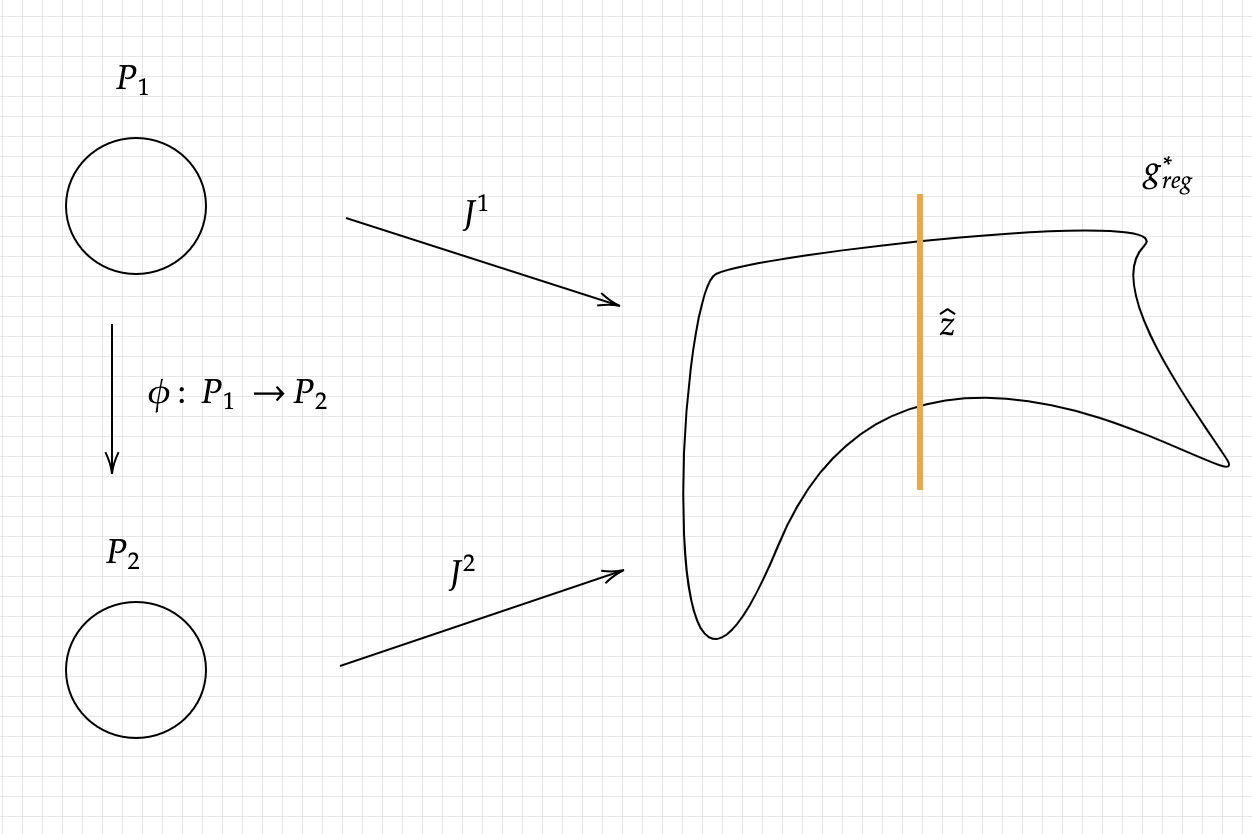
\includegraphics[width=0.4\linewidth]{Chapters/Figures/Screenshot 2025-03-07 at 1.40.07 PM.png}
    \caption{Existence of a $\mathrm{SO}(3)$-equivariant symplectomorphism $\phi$ comes from agreement of two moment maps, $J^{2}$ and $J^{1}$, such that the inverse images of $\hat{z}$ are acted on faithfully.}
    \label{fig:so3-symplectomorphism}
\end{figure}

\begin{proof}
Let $(P_{1}, \omega_{1}, \mathrm{SO}(3), J^{1})$ and $(P_{2}, \omega_{2}, \mathrm{SO}(3), J^{2})$ be two $4$-dimensional, compact Hamiltonian $\mathrm{SO}(3)$ spaces whose moment-images do not contain $0$. Let $F_{1}$ be a fibre of $\pi_{1}$. Then $\dim F_{1} + \dim \mathcal{O} = \dim P_{1}$ and $\dim F_{2} + \dim \mathcal{O} = \dim P_{2}$. By Delzant's Theorem, we have that that $\dim F_{1} = 2 \dim S^{1} = 2$. Furthermore, $\dim \mathcal{O} = 2$. Therefore, we require that $\dim P_{1} = \dim P_{2} = 4$. By \textit{Delzant's Theorem}, because both $S^{1}$ rotation actions are faithful with respect to the twisted action, the Delzant spaces $S^{1} \circlearrowright P_{1}$ and $S^{1} \circlearrowright P_{2}$ are symplectomorphic. By Theorem \ref{thm:hamiltonian-g-spaces-equivalence}, the $\mathrm{SO}(3)$ spaces are equivalent up to equivariant symplectomorphism by an element of $\mathrm{SO}(3)$. 
\end{proof} \bigskip 

\textbf{References}: \textcite{Delzant1988, Blaom1996}

